\documentclass{beamer}
\usepackage{lphs}
\usetikzlibrary{shapes,backgrounds}



\newcommand{\circA}[1]{
\begin{scope}[even odd rule]% first circle without the second
	\clip \secondcircle (-3,-3) rectangle (3,4) \thirdcircle(3,3);
	\fill[#1] \firstcircle;
\end{scope}}

\newcommand{\circB}[1]{
\begin{scope}[even odd rule]% first circle without the second
	\clip \thirdcircle (-3,-3) rectangle (3,4) \firstcircle(3,3);
	\fill[#1] \secondcircle;
\end{scope}}
	
\newcommand{\circC}[1]{
\begin{scope}[even odd rule]% first circle without the second
	\clip \firstcircle (-3,-3) rectangle (3,4) \secondcircle(3,3);
	\fill[#1] \thirdcircle;
\end{scope}}





\newcommand{\circAB}[1]{	
\begin{scope}
	\clip \firstcircle(3,3);
	\fill[#1] \secondcircle;
\end{scope}}
	
\newcommand{\circBC}[1]{	
\begin{scope}
	\clip \thirdcircle(3,3);
	\fill[#1] \secondcircle;
\end{scope}}

\newcommand{\circAC}[1]{	
\begin{scope}
	\clip \thirdcircle(3,3);
	\fill[#1] \firstcircle;
\end{scope}}

\newcommand{\circABC}[1]{
\begin{scope}
	\clip \thirdcircle(3,3);
	\clip \secondcircle(3,3);
	\fill[#1] \firstcircle;
\end{scope}}



\begin{document}
	
	
\begin{frame}

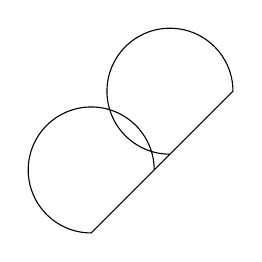
\begin{tikzpicture}
\draw (0,0) arc (0:270:8mm) -- (1,1) arc (0:270:8mm);
\end{tikzpicture}

\end{frame}

\begin{frame}

\newcommand{\firstcircle}{(-1,0) circle (1.5)}
\newcommand{\secondcircle}{(1,0) circle (1.5)}
\newcommand{\thirdcircle}{(0,1.73) circle (1.5)}


% Now we can draw the sets:
\begin{tikzpicture}

\fill[gray] \firstcircle;
\fill[gray] \secondcircle;


\circA{red}


\draw \firstcircle node {A};
\draw \secondcircle node {B};

\end{tikzpicture}

\end{frame}	
\end{document}